\documentclass[12pt, border=8pt]{standalone}
\usepackage{tikz}
\usepackage{amsmath, amssymb, bm}
\usepackage{xcolor}
\usetikzlibrary{positioning, arrows.meta, calc, fit, backgrounds}

\begin{document}


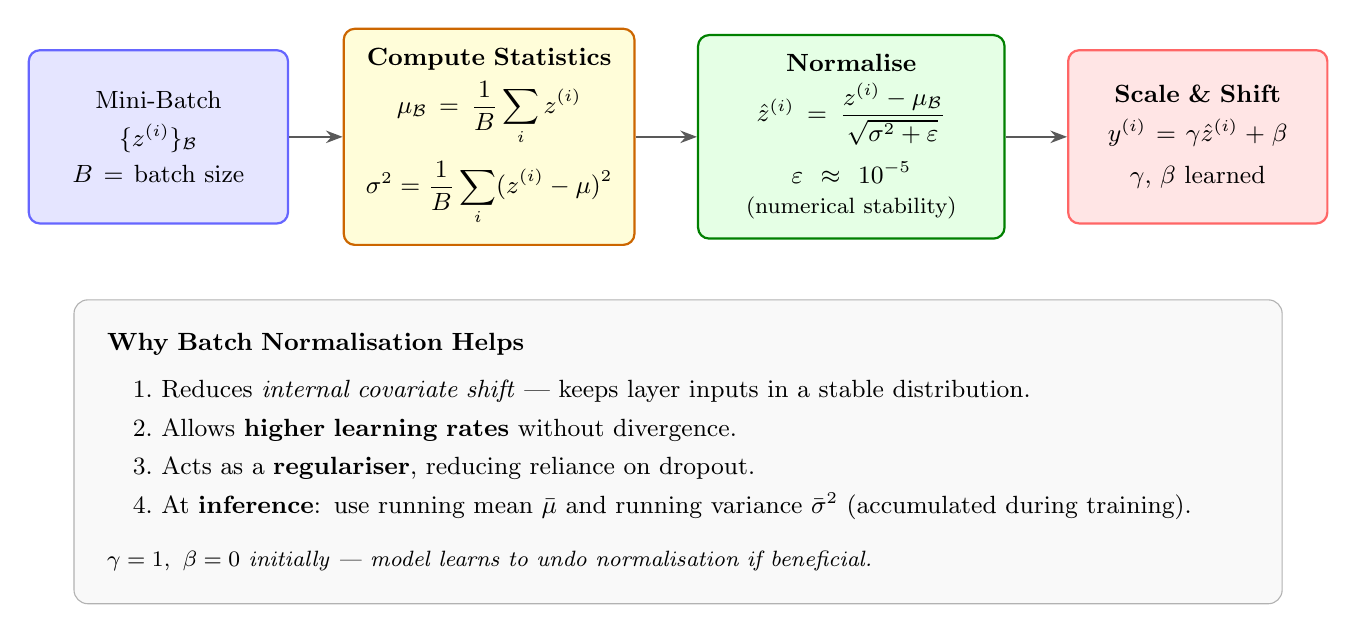
\begin{tikzpicture}[
  batchbox/.style={
    rectangle, draw=blue!60, fill=blue!10, thick,
    rounded corners=4pt, text width=2.8cm, align=center,
    minimum height=2.2cm, font=\small, inner sep=7pt
  },
  statsbox/.style={
    rectangle, draw=orange!80!black, fill=yellow!15, thick,
    rounded corners=4pt, text width=3.2cm, align=center,
    minimum height=2.2cm, font=\small, inner sep=7pt
  },
  normbox/.style={
    rectangle, draw=green!50!black, fill=green!10, thick,
    rounded corners=4pt, text width=3.4cm, align=center,
    minimum height=2.2cm, font=\small, inner sep=7pt
  },
  scalebox/.style={
    rectangle, draw=red!60, fill=red!10, thick,
    rounded corners=4pt, text width=2.8cm, align=center,
    minimum height=2.2cm, font=\small, inner sep=7pt
  },
  pipe/.style={-{Stealth[length=6pt]}, gray!70!black, thick},
]

%% ── Pipeline boxes ───────────────────────────────────────────────────────────
\node[batchbox] (batch) at (0, 0) {%
  Mini-Batch\\[3pt]
  $\{z^{(i)}\}_{\mathcal{B}}$\\[2pt]
  $B = \text{batch size}$
};

\node[statsbox] (stats) at (4.2, 0) {%
  \textbf{Compute Statistics}\\[3pt]
  $\mu_{\mathcal{B}} = \dfrac{1}{B}\displaystyle\sum_{i} z^{(i)}$\\[5pt]
  $\sigma^2 = \dfrac{1}{B}\displaystyle\sum_{i}(z^{(i)}-\mu)^2$
};

\node[normbox] (norm) at (8.8, 0) {%
  \textbf{Normalise}\\[3pt]
  $\hat{z}^{(i)} = \dfrac{z^{(i)}-\mu_{\mathcal{B}}}{\sqrt{\sigma^2+\varepsilon}}$\\[5pt]
  $\varepsilon \approx 10^{-5}$\\
  {\footnotesize(numerical stability)}
};

\node[scalebox] (scale) at (13.2, 0) {%
  \textbf{Scale \& Shift}\\[3pt]
  $y^{(i)} = \gamma\hat{z}^{(i)} + \beta$\\[4pt]
  $\gamma,\,\beta$ learned
};

%% ── Arrows ───────────────────────────────────────────────────────────────────
\draw[pipe] (batch.east) -- (stats.west);
\draw[pipe] (stats.east) -- (norm.west);
\draw[pipe] (norm.east)  -- (scale.west);

%% ── "Why BN Helps" box ───────────────────────────────────────────────────────
\node[
  draw=gray!60, fill=gray!5, rounded corners=5pt,
  text width=14.5cm, align=left,
  inner sep=12pt, font=\small
] (whybox) at (6.6, -4.0) {%
  \textbf{Why Batch Normalisation Helps}\\[6pt]
  \quad 1.\ Reduces \emph{internal covariate shift} --- keeps layer inputs in a stable distribution.\\[3pt]
  \quad 2.\ Allows \textbf{higher learning rates} without divergence.\\[3pt]
  \quad 3.\ Acts as a \textbf{regulariser}, reducing reliance on dropout.\\[3pt]
  \quad 4.\ At \textbf{inference}: use running mean $\bar{\mu}$ and running variance $\bar{\sigma}^2$
            (accumulated during training).\\[8pt]
  \footnotesize
  \textit{$\gamma = 1,\ \beta = 0$ initially ---
  model learns to undo normalisation if beneficial.}
};

\end{tikzpicture}

\end{document}
